\chapter{Shannon Capacity and Performance Gap}

\section{Shannon Capacity}
The Shannon capacity of a communication channel is given by
\[
C = B \log_2(1+\text{SNR})
\]
where \(B\) is the communication bandwidth in Hz.

For this batch, the bandwidth is
\[
B = 2R_b
\]
Since the assigned bit rate is \(R_b = 1~\text{kbps}\), the bandwidth becomes
\[
B = 2 \times 1000 = 2000~\text{Hz}
\]

Thus, the channel capacity depends on both bandwidth and signal-to-noise ratio. As SNR increases, the achievable data rate increases, but the gain becomes slower at high SNR values.
\newpage
\section{Python Implementation}
The following code computes and plots Shannon capacity versus SNR.

\begin{lstlisting}[style=pythonstyle, caption={Shannon Capacity Calculation and Plot}]
import numpy as np
import matplotlib.pyplot as plt

Rb = 1000
B = 2 * Rb

SNRdB = np.arange(0, 21, 2)
SNRlinear = 10**(SNRdB / 10)
C = B * np.log2(1 + SNRlinear)

plt.figure(figsize=(8,5))
plt.plot(SNRdB, C, 'o-', color='purple')
plt.xlabel('SNR (dB)')
plt.ylabel('Capacity (bps)')
plt.title('Shannon Capacity versus SNR')
plt.grid(True)
plt.tight_layout()
plt.show()
\end{lstlisting}

\section{Performance Gap from Shannon Limit}
For uncoded BPSK, the approximate \(E_b/N_0\) required to achieve a BER of \(10^{-5}\) is \(9.6\) dB. The Shannon limit reference is \(1.59\) dB. Therefore, the performance gap is
\[
\text{Gap} = 9.6 - 1.59 = 8.01~\text{dB}
\]

This gap shows that practical uncoded BPSK requires much more energy per bit than the theoretical minimum allowed by Shannon capacity. The reason is that uncoded systems do not use redundancy efficiently to combat noise.

\section{Discussion}
The Shannon capacity curve shows that channel capacity increases with SNR, but the improvement becomes gradual at higher values. This means that simply increasing power is not always an efficient way to improve communication performance.

The gap between practical BPSK and the Shannon limit can be reduced using forward error correction methods such as LDPC and Turbo codes. These coding techniques add structured redundancy, which helps the receiver correct errors with lower transmitted power.

\begin{figure}[htbp]
    \centering
    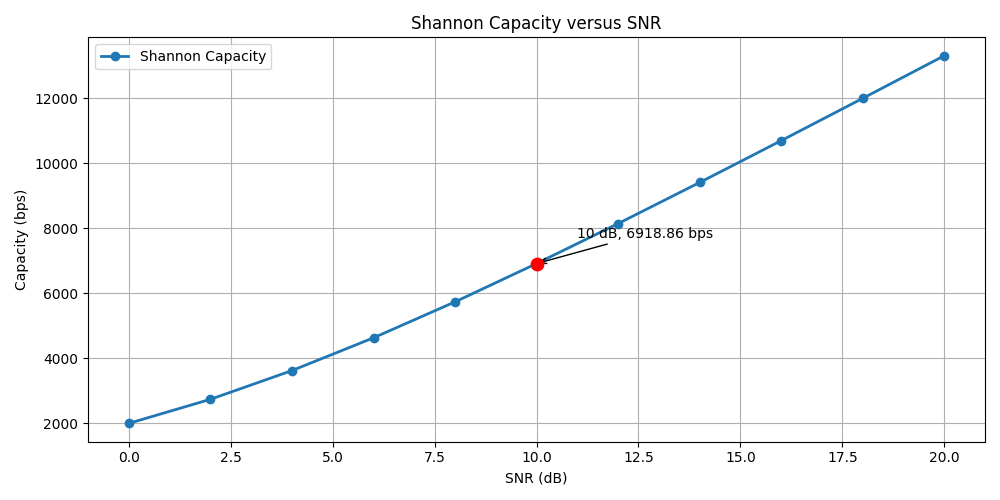
\includegraphics[width=0.8\textwidth]{./plots/shannon_capacity_vs_snr.png}
    \caption{Shannon capacity versus SNR}
\end{figure}

\section{Conclusion}
The capacity analysis confirms that both bandwidth and SNR control the maximum possible data rate of the channel. The calculated gap from the Shannon limit highlights the difference between ideal information-theoretic performance and practical uncoded BPSK operation.